%%%%%%%%%%%%%%%%%%%%%%%%%%%%%%%%%% NAME %%%%%%%%%%%%%%%%%%%%%%%%%%%%%
%%%%%%%%%%%%%%%%%
\section{Introduction}
%%%%%%%%%%%%%%%%%
%%%%%%%%%%%%%%%%
\subsection{Robotic Lawn mowers}

\begin{frame}{Introduction}{Robotic Lawn mowers}
  \begin{figure}
    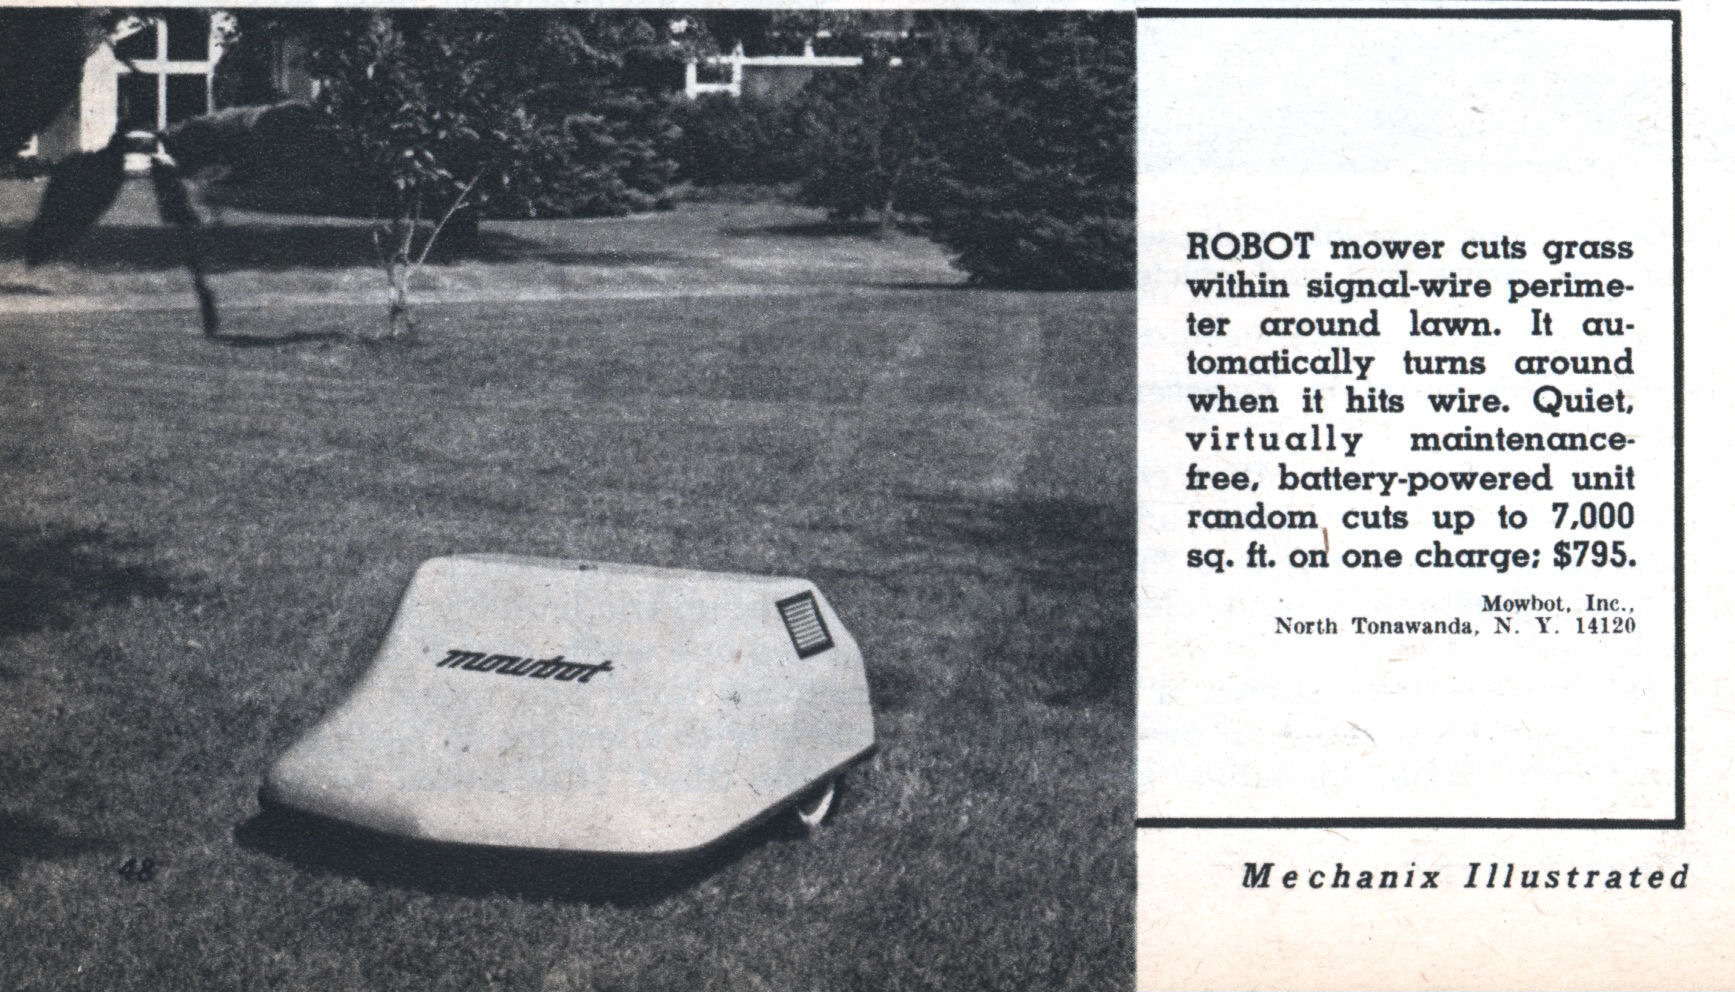
\includegraphics[width=\linewidth]{Pictures/mowbot.jpg}
  \end{figure}
\pause
$$\$795 (1969) \approx \$5296 (2016)$$
\end{frame}
%%%%%%%%%%%%%%%%

%%%%%%%%%%%%%%%%
\subsection{Navigation}

\begin{frame}{Introduction}{Navigation}
    \begin{figure}[!htb]
    \centering
    \begin{minipage}{.8\textwidth}
        \centering
        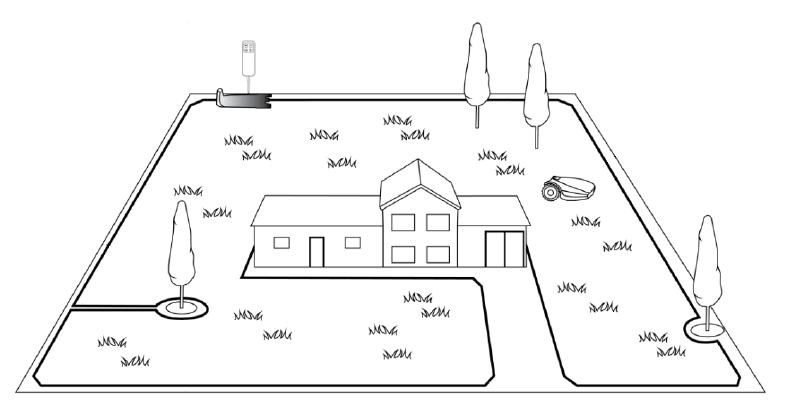
\includegraphics[width=0.99\linewidth]{Pictures/robomow.png}
    \end{minipage}%
    \begin{minipage}{0.2\textwidth}
        \centering
        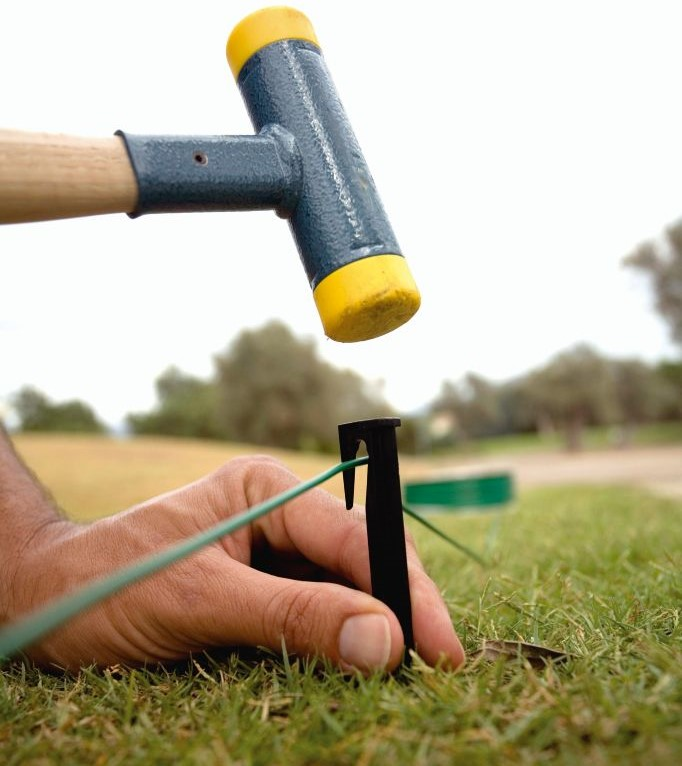
\includegraphics[width=0.99\linewidth]{Pictures/wirehammer.jpg}
    \end{minipage}  
    \end{figure}
\end{frame}
\begin{frame}{Introduction}{Navigation}
    \begin{figure}[!htb]
    \centering
        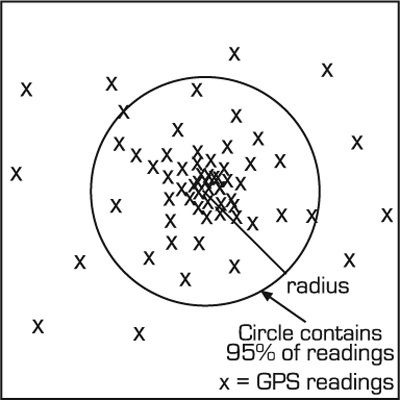
\includegraphics[width=0.7\linewidth]{Pictures/gps.jpg}
    \end{figure}
\end{frame}

%%%%%%%%%%%%%%%%

%%%%%%%%%%%%%%%%
\subsection{Cutting strategies}

\begin{frame}{Introduction}{Cutting strategies}
  Two main types:
 

  \begin{figure}[!htb]
    \centering
    \begin{minipage}{.5\textwidth}
        \centering
        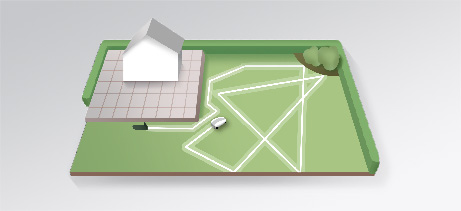
\includegraphics[width=0.99\linewidth]{Pictures/noLogiCut.jpg}
    \end{minipage}%
    \begin{minipage}{0.5\textwidth}
        \centering
        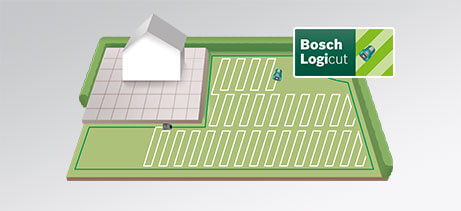
\includegraphics[width=0.99\linewidth]{Pictures/logicut.jpg}
    \end{minipage}
\end{figure}
\vspace{-20pt}
  \begin{table}
   \begin{tabular*}{\columnwidth}{@{\extracolsep{38pt}}cc}
  1. Random direction & 2. Parallel line \\ 
  \end{tabular*} 
\end{table} 

\end{frame}
%%%%%%%%%%%%%%%%


%%%%%%%%%%%%%%%%%%%%%%%%%%%%%%%%%% NAME %%%%%%%%%%%%%%%%%%%%%%%%%%%%%
%%%%%%%%%%%%%%%%%
\section{Design Considerations}
%%%%%%%%%%%%%%%%%

%%%%%%%%%%%%%%%%
\subsection{Use-case Design}

\begin{frame}{Design Considerations}{Use-case Design}
\begin{figure}
\centering
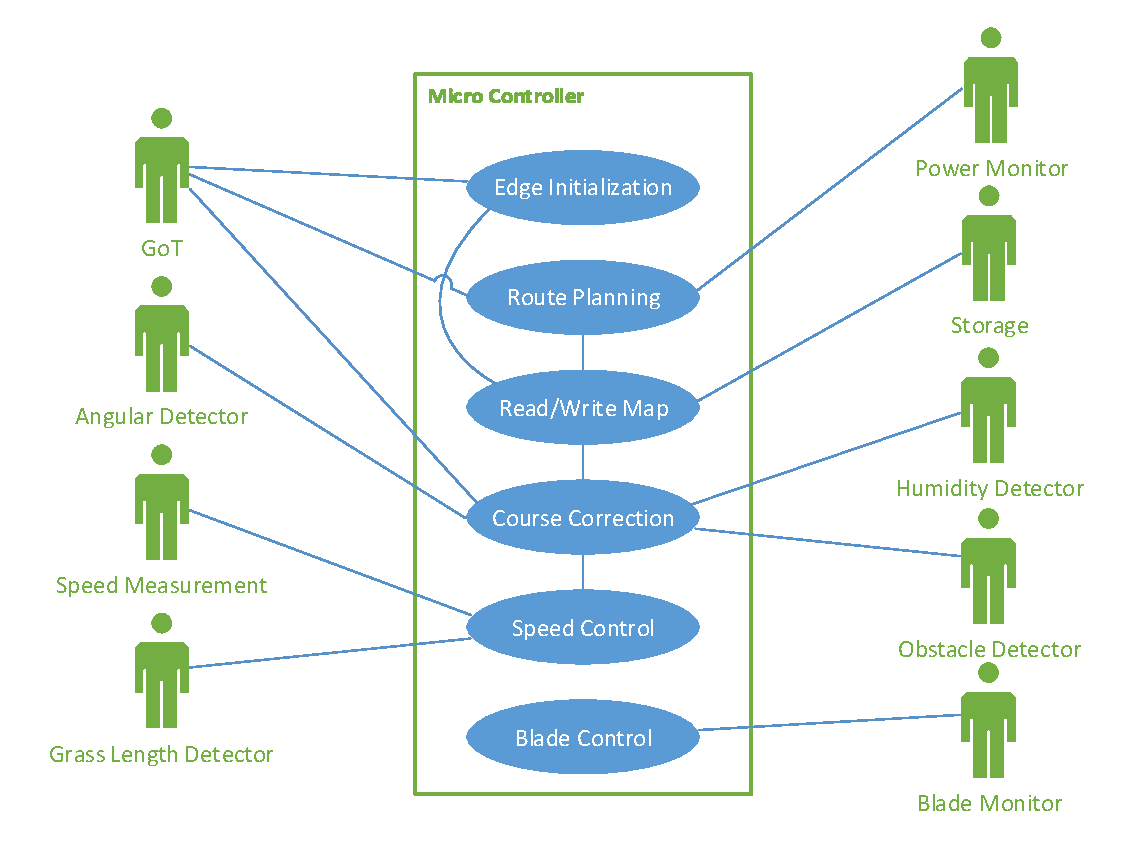
\includegraphics[width=\linewidth]{Pictures/P5UseCase.pdf}
\end{figure}
\end{frame}
%%%%%%%%%%%%%%%%

%%%%%%%%%%%%%%%%
\subsection{Prototype Vehicle}

\begin{frame}{Design Considerations}{Prototype Vehicle}
\begin{figure}
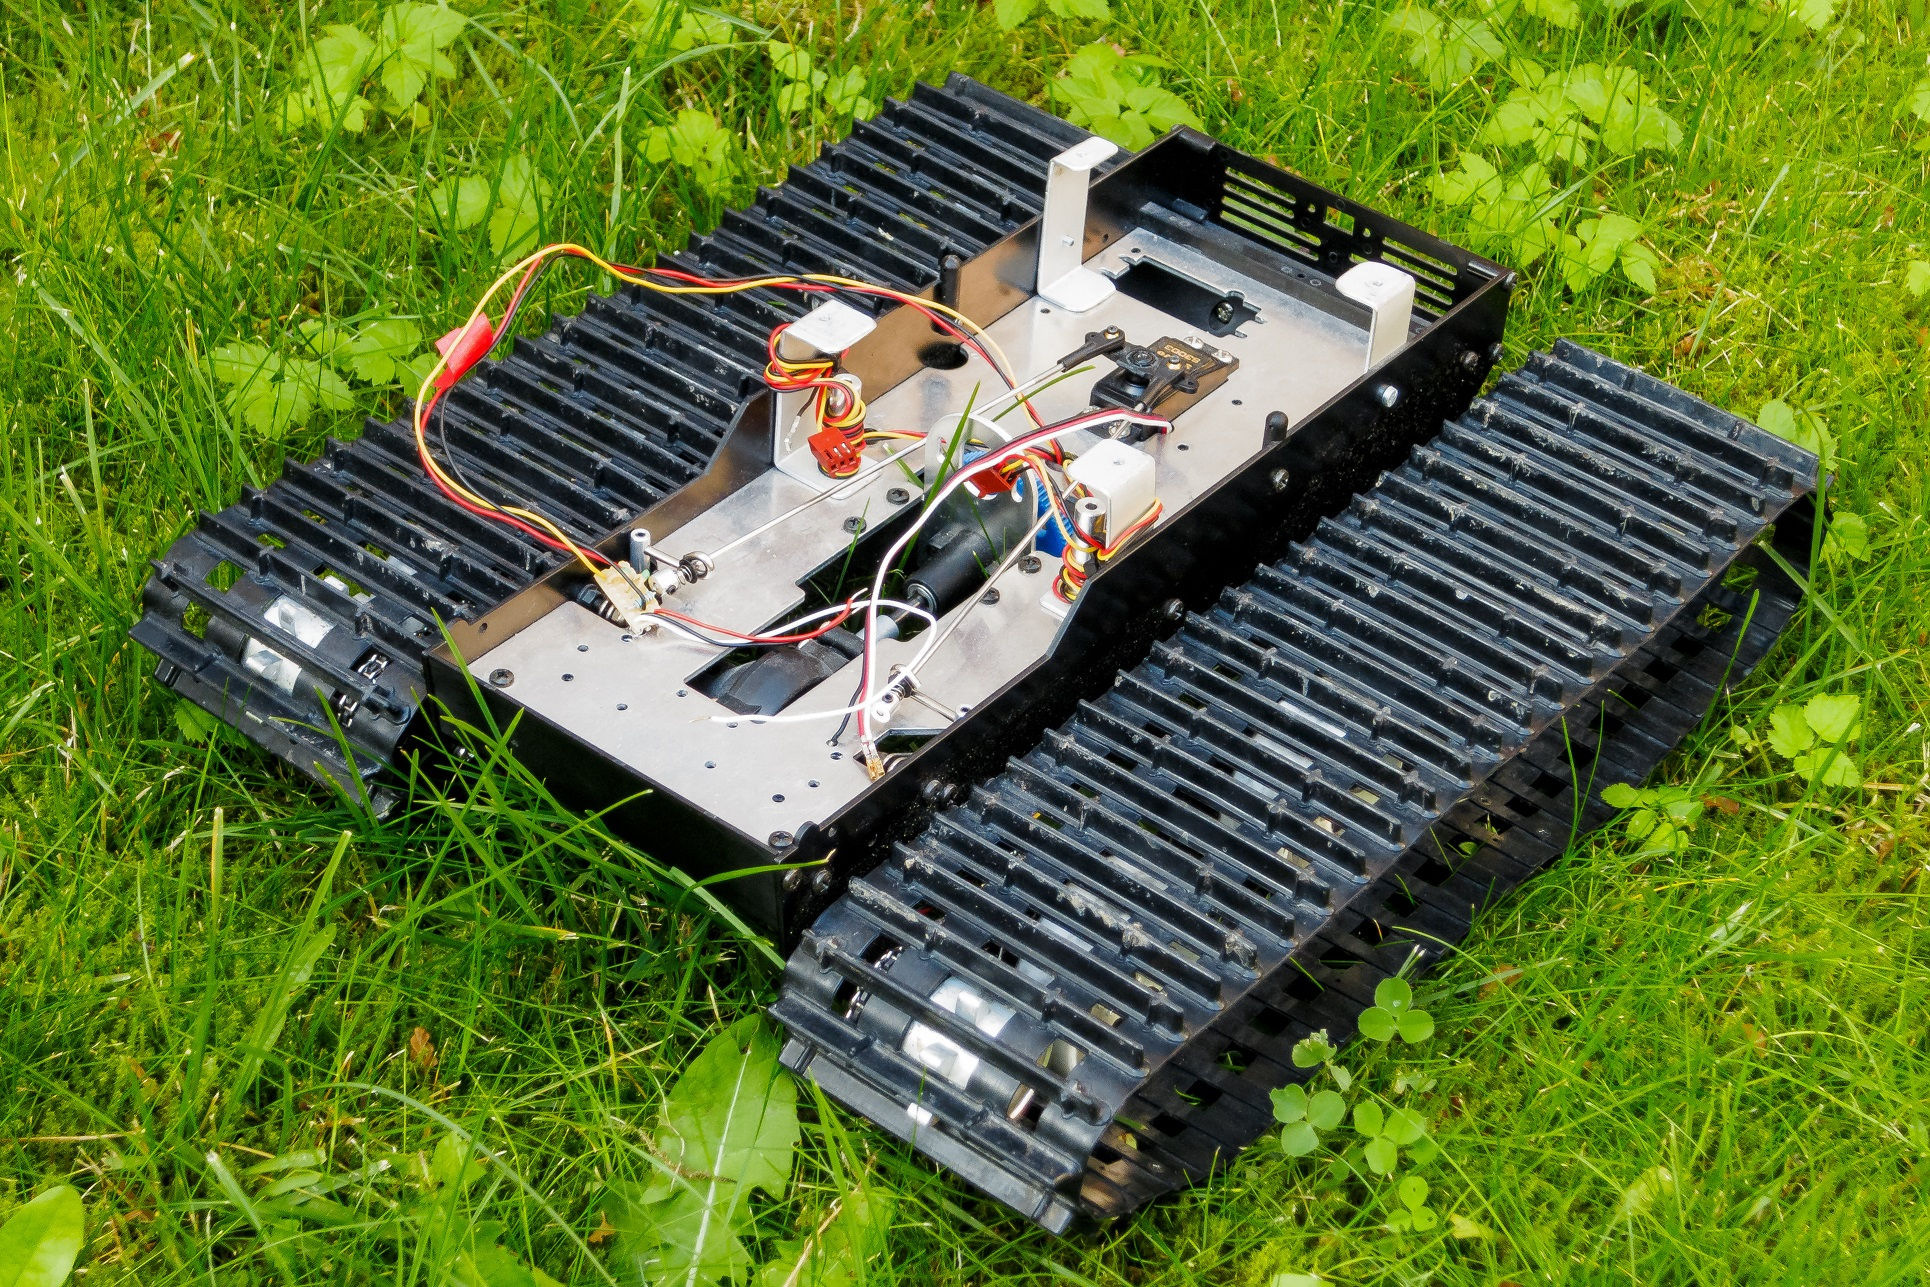
\includegraphics[width=\textwidth]{Pictures/BeltVehicle.jpg}
\end{figure}
\end{frame}
\begin{frame}{Design Considerations}{Prototype Vehicle}
\begin{figure}
\includegraphics[width=\textwidth]{Pictures/FullVehicle.png}
\end{figure}
\end{frame}


\section{Prototype Requirements}
\begin{frame}{Prototype Requirements}
\begin{figure}
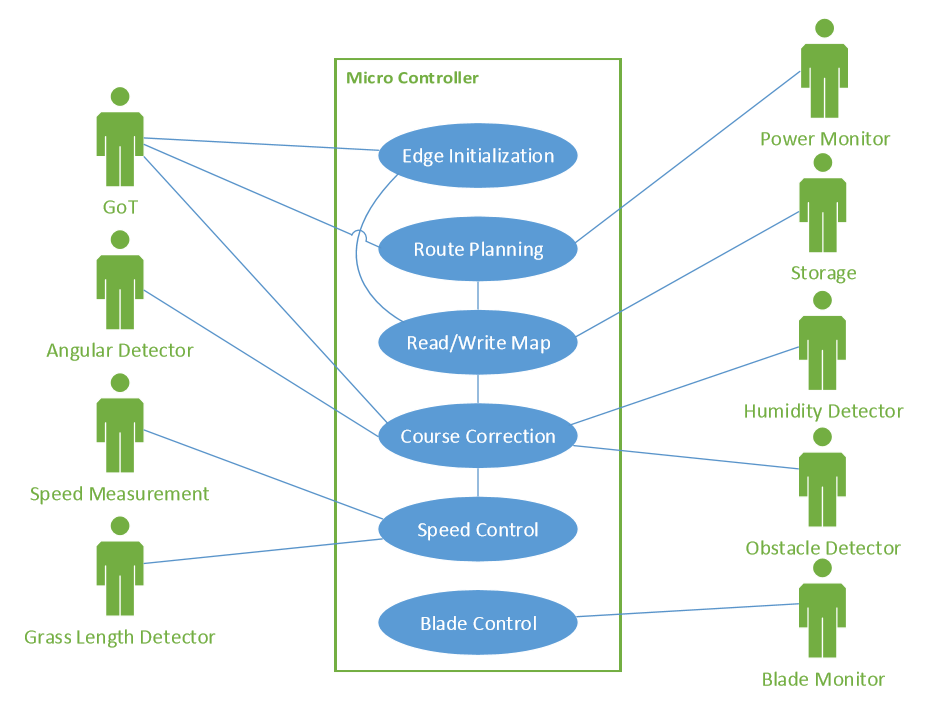
\includegraphics[width=\textwidth]{Pictures/uc1.png}
\end{figure}
\end{frame}
\begin{frame}{Prototype Requirements}
\begin{figure}
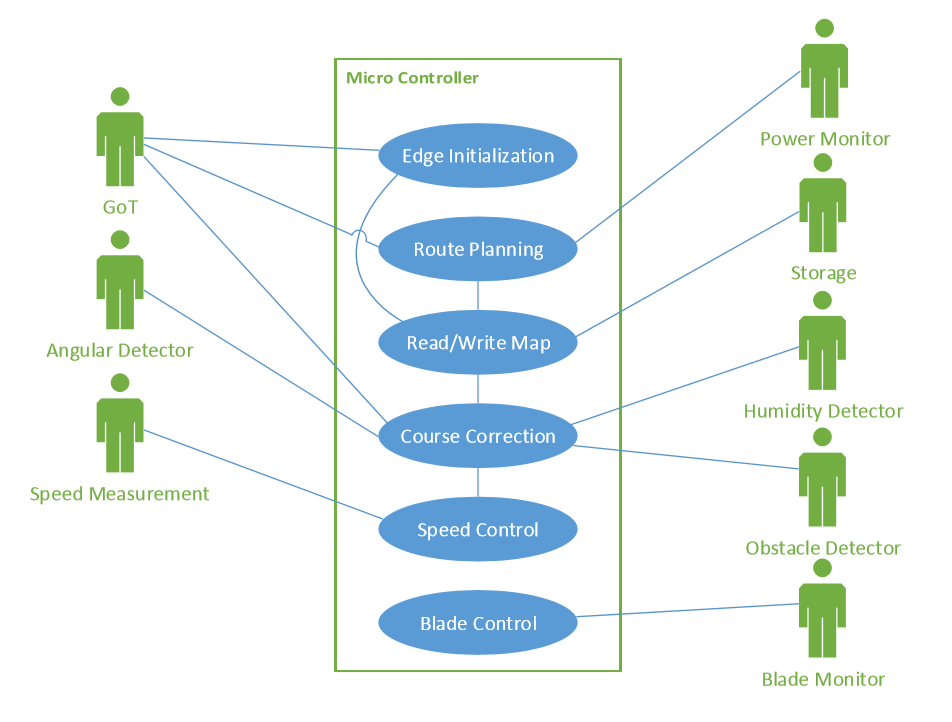
\includegraphics[width=\textwidth]{Pictures/uc2.png}
\end{figure}
\end{frame}
\begin{frame}{Prototype Requirements}
\begin{figure}
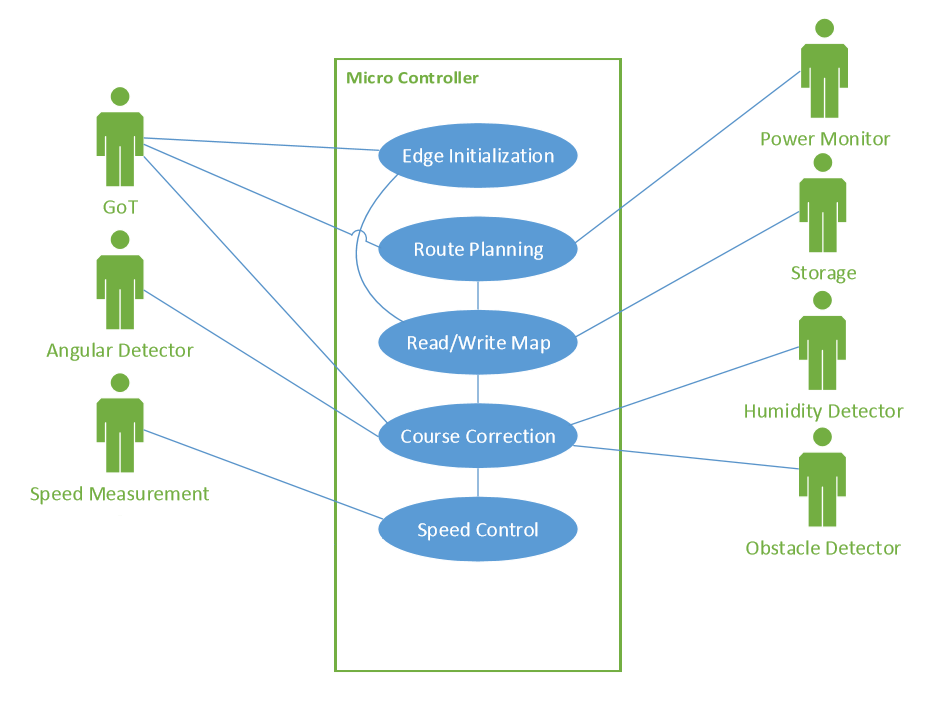
\includegraphics[width=\textwidth]{Pictures/uc3.png}
\end{figure}
\end{frame}
\begin{frame}{Prototype Requirements}
\begin{figure}
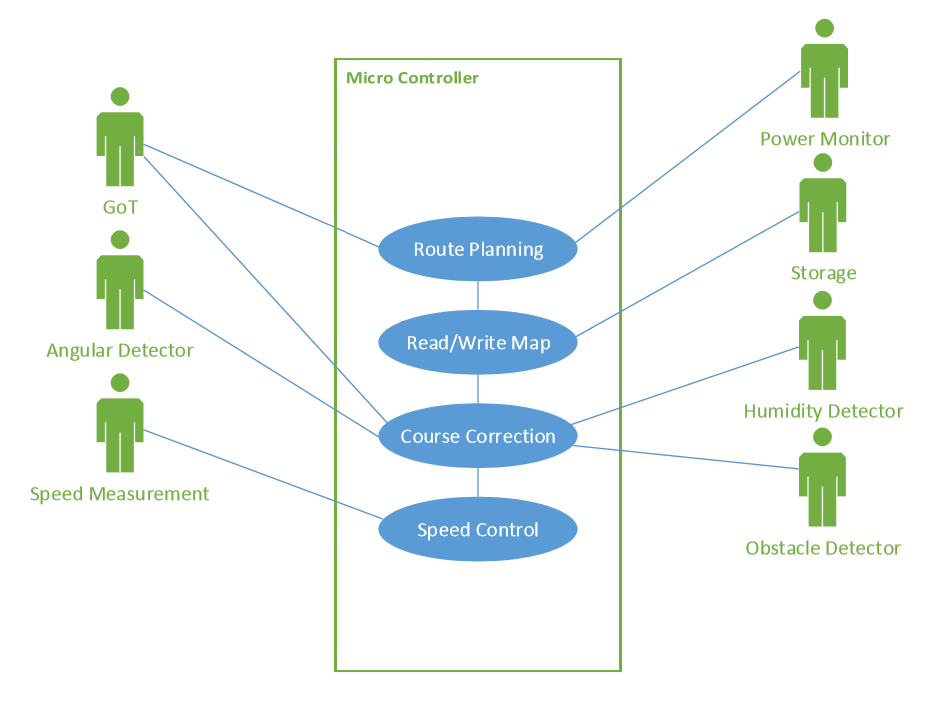
\includegraphics[width=\textwidth]{Pictures/uc4.png}
\end{figure}
\end{frame}
\begin{frame}{Prototype Requirements}
\begin{figure}
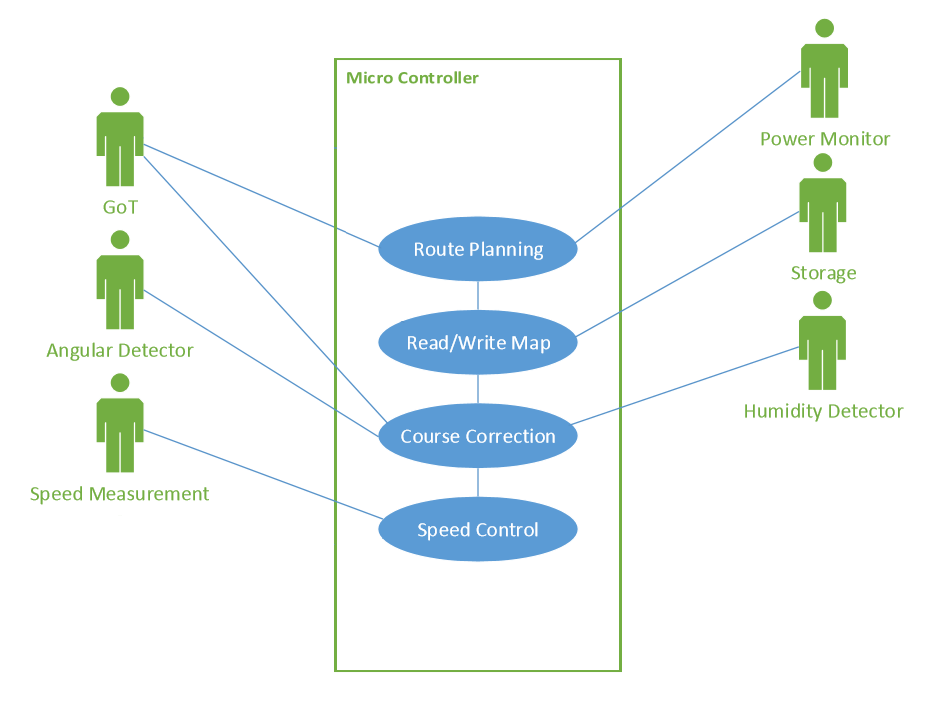
\includegraphics[width=\textwidth]{Pictures/uc5.png}
\end{figure}
\end{frame}
\begin{frame}{Prototype Requirements}
\begin{figure}
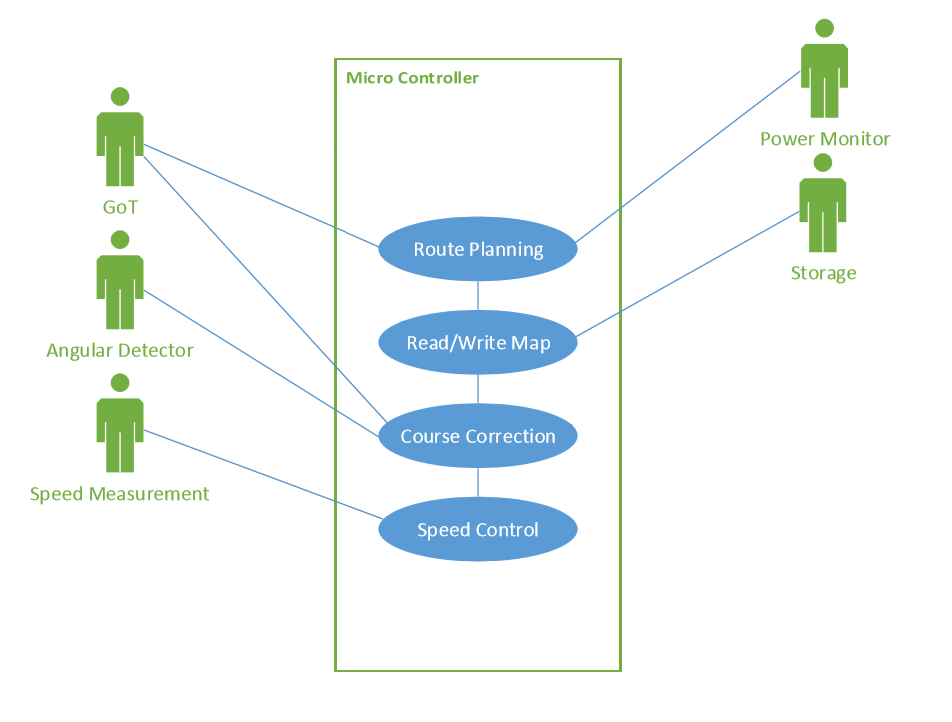
\includegraphics[width=\textwidth]{Pictures/uc6.png}
\end{figure}
\end{frame}
%%%%%%%%%%%%%%%%
%%%%%%%%%%%%%%%%%%%%%%%%%%%%%%%%%% NAME %%%%%%%%%%%%%%%%%%%%%%%%%%%%%
%%%%%%%%%%%%%%%%%


\begin{frame}{Prototype Requirements}
  \begin{enumerate}
\footnotesize
\item \textbf{It shall be possible for the vehicle to receive its own location wirelessly from the GoT system, through a computer.}
\item \textbf{It shall be possible for the prototype to disregard incorrect packets transmitted from the computer}
	\item \textbf{The prototype must be able to disregard erroneous coordinates sent from the GoT system}
\item \textbf{The prototype must be able to access the route, which it has to follow, from a storage space located on the vehicle}
\item \textbf{The prototype must be able to shut down, if the battery voltage is below its cut-off specification}
\item \textbf{It shall be possible for the prototype to follow a predetermined route}
\item \textbf{It shall be possible for the prototype to return to the predetermined route if disturbed}
\item \textbf{The prototype shall be able to keep a velocity on 1,4 $m \cdot s^{-1}$, when going up - or downhill and when turning}
\end{enumerate}
\end{frame}
%%%%%%%%%%%%%%%%%
